\begin{tikzpicture}
  \node at (-2, 0) {}; % force left edge here
  \Tree [.\node[fill=yellow,fill opacity=0,text opacity=1,color=black](S){S};
          [.\node[fill=yellow,fill opacity=0,text opacity=1,color=black](NP1){$\text{NP}_1$};
            \node[fill=yellow,fill opacity=0,text opacity=1,color=black](The){The};
            \node[fill=yellow,fill opacity=0,text opacity=1,color=black](man){man}; ]
          [.\node[fill=yellow,fill opacity=0,text opacity=1,color=black]{VP};
            [.\node[fill=yellow,fill opacity=0,text opacity=1,color=black](picked){picked}; ]
            [.\node[fill=yellow,fill opacity=0,text opacity=1,color=black](NP2){$\text{NP}_2$};
              \node[fill=yellow,fill opacity=0,text opacity=1,color=black]{the};
              \node[fill=yellow,fill opacity=0,text opacity=1,color=black]{vegetables}; ] ] ];
%  \node [anchor=west] (cmd) at (4.5, 0) {\textsc{Shift}};
  \draw (4.4, -0.25) rectangle (6.5, -0.75);
  \draw (4.4, -0.75) rectangle (6.5, -1.25);
  \draw [fill=none] (4.4, -1.25) rectangle (6.5, -1.75);
  \draw [fill=none] (4.4, -1.75) rectangle (6.5, -2.25);
%  \node [anchor=west] (s4) at (4.5, -0.5) {vegetables};
%  \node [anchor=west] (s3) at (4.5, -1) {};
%  \node [anchor=west] (s2) at (4.5, -1.5) {The};
%  \node [anchor=west] (s1) at (4.5, -2) {man};
\end{tikzpicture}

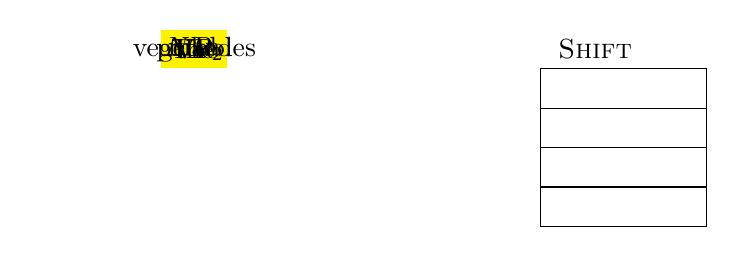
\begin{tikzpicture}
  \node at (-2, 0) {}; % force left edge here
  \Tree [.\node[fill=yellow,fill opacity=0,text opacity=1](S){\color{black} S};
          [.\node[fill=yellow,fill opacity=0,text opacity=1](NP1){\color{black} $\text{NP}_1$};
            \node[fill=yellow,fill opacity=1,text opacity=1](The){\color{black} The};
            \node[fill=yellow,fill opacity=0,text opacity=1](man){\color{black} man}; ]
          [.\node[fill=yellow,fill opacity=0,text opacity=1]{\color{black} VP};
            [.\node[fill=yellow,fill opacity=0,text opacity=1](picked){\color{black} picked}; ]
            [.\node[fill=yellow,fill opacity=0,text opacity=1](NP2){\color{black} $\text{NP}_2$};
              \node[fill=yellow,fill opacity=0,text opacity=1]{\color{black} the};
              \node[fill=yellow,fill opacity=0,text opacity=1]{\color{black} vegetables}; ] ] ];
  \node [anchor=west] (cmd) at (4.5, 0) {\textsc{Shift}};
  \draw (4.4, -0.25) rectangle (6.5, -0.75);
  \draw (4.4, -0.75) rectangle (6.5, -1.25);
  \draw [fill=none] (4.4, -1.25) rectangle (6.5, -1.75);
  \draw [fill=none] (4.4, -1.75) rectangle (6.5, -2.25);
%  \node [anchor=west] (s4) at (4.5, -0.5) {vegetables};
%  \node [anchor=west] (s3) at (4.5, -1) {};
%  \node [anchor=west] (s2) at (4.5, -1.5) {The};
%  \node [anchor=west] (s1) at (4.5, -2) {man};
\end{tikzpicture}

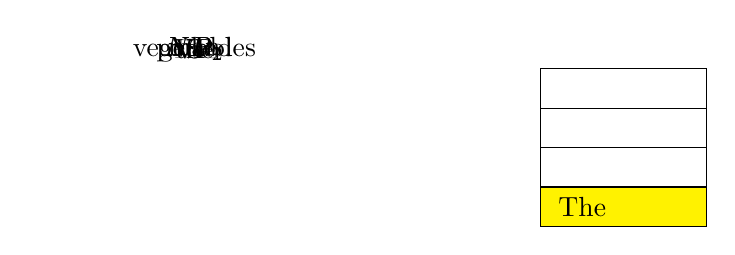
\begin{tikzpicture}
  \node at (-2, 0) {}; % force left edge here
  \Tree [.\node[fill=yellow,fill opacity=0,text opacity=1](S){\color{black} S};
          [.\node[fill=yellow,fill opacity=0,text opacity=1](NP1){\color{black} $\text{NP}_1$};
            \node[fill=yellow,fill opacity=0,text opacity=1](The){\color{gray} The};
            \node[fill=yellow,fill opacity=0,text opacity=1](man){\color{black} man}; ]
          [.\node[fill=yellow,fill opacity=0,text opacity=1]{\color{black} VP};
            [.\node[fill=yellow,fill opacity=0,text opacity=1](picked){\color{black} picked}; ]
            [.\node[fill=yellow,fill opacity=0,text opacity=1](NP2){\color{black} $\text{NP}_2$};
              \node[fill=yellow,fill opacity=0,text opacity=1]{\color{black} the};
              \node[fill=yellow,fill opacity=0,text opacity=1]{\color{black} vegetables}; ] ] ];
%  \node [anchor=west] (cmd) at (4.5, 0) {\textsc{Shift}};
  \draw (4.4, -0.25) rectangle (6.5, -0.75);
  \draw (4.4, -0.75) rectangle (6.5, -1.25);
  \draw [fill=none] (4.4, -1.25) rectangle (6.5, -1.75);
  \draw [fill=yellow] (4.4, -1.75) rectangle (6.5, -2.25);
%  \node [anchor=west] (s4) at (4.5, -0.5) {vegetables};
%  \node [anchor=west] (s3) at (4.5, -1) {};
%  \node [anchor=west] (s2) at (4.5, -1.5) {The};
  \node [anchor=west] (s1) at (4.5, -2) {The};
\end{tikzpicture}

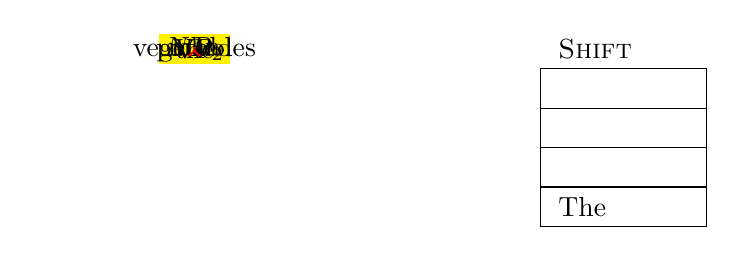
\begin{tikzpicture}
  \node at (-2, 0) {}; % force left edge here
  \Tree [.\node[fill=yellow,fill opacity=0,text opacity=1](S){\color{black} S};
          [.\node[fill=yellow,fill opacity=0,text opacity=1](NP1){\color{black} $\text{NP}_1$};
            \node[fill=yellow,fill opacity=0,text opacity=1](The){\color{gray} The};
            \node[fill=yellow,fill opacity=1,text opacity=1](man){\color{black} man}; ]
          [.\node[fill=yellow,fill opacity=0,text opacity=1](VP){\color{black} VP};
            [.\node[fill=yellow,fill opacity=0,text opacity=1](picked){\color{black} picked}; ]
            [.\node[fill=yellow,fill opacity=0,text opacity=1](NP2){\color{black} $\text{NP}_2$};
              \node[fill=yellow,fill opacity=0,text opacity=1](the2){\color{black} the};
              \node[fill=yellow,fill opacity=0,text opacity=1](vegetables){\color{black} vegetables}; ] ] ];
  \node [anchor=west] (cmd) at (4.5, 0) {\textsc{Shift}};
  \draw (4.4, -0.25) rectangle (6.5, -0.75);
  \draw (4.4, -0.75) rectangle (6.5, -1.25);
  \draw [fill=none] (4.4, -1.25) rectangle (6.5, -1.75);
  \draw [fill=none] (4.4, -1.75) rectangle (6.5, -2.25);
%  \node [anchor=west] (s4) at (4.5, -0.5) {vegetables};
%  \node [anchor=west] (s3) at (4.5, -1) {};
%  \node [anchor=west] (s2) at (4.5, -1.5) {The};
  \node [anchor=west] (s1) at (4.5, -2) {The};
  \draw [->, thick, red] (The.center) -- (man.center);
\end{tikzpicture}

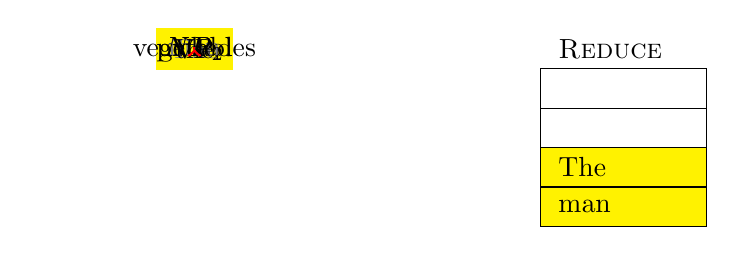
\begin{tikzpicture}
  \node at (-2, 0) {}; % force left edge here
  \Tree [.\node[fill=yellow,fill opacity=0,text opacity=1](S){\color{black} S};
          [.\node[fill=yellow,fill opacity=1,text opacity=1](NP1){\color{black} $\text{NP}_1$};
            \node[fill=yellow,fill opacity=0,text opacity=1](The){\color{gray} The};
            \node[fill=yellow,fill opacity=0,text opacity=1](man){\color{gray} man}; ]
          [.\node[fill=yellow,fill opacity=0,text opacity=1]{\color{black} VP};
            [.\node[fill=yellow,fill opacity=0,text opacity=1](picked){\color{black} picked}; ]
            [.\node[fill=yellow,fill opacity=0,text opacity=1](NP2){\color{black} $\text{NP}_2$};
              \node[fill=yellow,fill opacity=0,text opacity=1]{\color{black} the};
              \node[fill=yellow,fill opacity=0,text opacity=1]{\color{black} vegetables}; ] ] ];
  \node [anchor=west] (cmd) at (4.5, 0) {\textsc{Reduce}};
  \draw (4.4, -0.25) rectangle (6.5, -0.75);
  \draw (4.4, -0.75) rectangle (6.5, -1.25);
  \draw [fill=yellow] (4.4, -1.25) rectangle (6.5, -1.75);
  \draw [fill=yellow] (4.4, -1.75) rectangle (6.5, -2.25);
%  \node [anchor=west] (s4) at (4.5, -0.5) {vegetables};
%  \node [anchor=west] (s3) at (4.5, -1) {};
  \node [anchor=west] (s2) at (4.5, -1.5) {The};
  \node [anchor=west] (s1) at (4.5, -2) {man};
  \draw [->, thick, red] (The.center) -- (man.center);
  \draw [->, thick, red] (man.center) -- (NP1.center);
\end{tikzpicture}

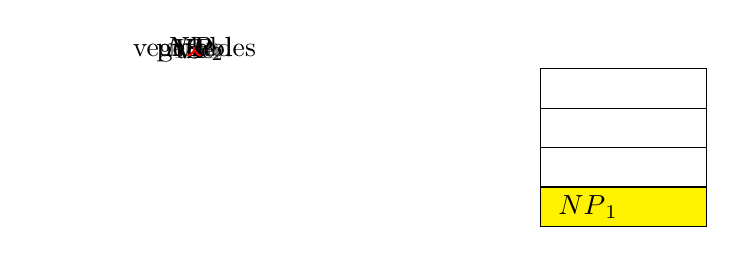
\begin{tikzpicture}
  \node at (-2, 0) {}; % force left edge here
  \Tree [.\node[fill=yellow,fill opacity=0,text opacity=1](S){\color{black} S};
          [.\node[fill=yellow,fill opacity=0,text opacity=1](NP1){\color{gray} $\text{NP}_1$};
            \node[fill=yellow,fill opacity=0,text opacity=1](The){\color{gray} The};
            \node[fill=yellow,fill opacity=0,text opacity=1](man){\color{gray} man}; ]
          [.\node[fill=yellow,fill opacity=0,text opacity=1]{\color{black} VP};
            [.\node[fill=yellow,fill opacity=0,text opacity=1](picked){\color{black} picked}; ]
            [.\node[fill=yellow,fill opacity=0,text opacity=1](NP2){\color{black} $\text{NP}_2$};
              \node[fill=yellow,fill opacity=0,text opacity=1]{\color{black} the};
              \node[fill=yellow,fill opacity=0,text opacity=1]{\color{black} vegetables}; ] ] ];
%  \node [anchor=west] (cmd) at (4.5, 0) {\textsc{Reduce}};
  \draw (4.4, -0.25) rectangle (6.5, -0.75);
  \draw (4.4, -0.75) rectangle (6.5, -1.25);
  \draw [fill=none] (4.4, -1.25) rectangle (6.5, -1.75);
  \draw [fill=yellow] (4.4, -1.75) rectangle (6.5, -2.25);
%  \node [anchor=west] (s4) at (4.5, -0.5) {vegetables};
%  \node [anchor=west] (s3) at (4.5, -1) {};
%  \node [anchor=west] (s2) at (4.5, -1.5) {The};
  \node [anchor=west] (s1) at (4.5, -2) {$\text{NP}_1$};
  \draw [->, thick, red] (The.center) -- (man.center);
  \draw [->, thick, red] (man.center) -- (NP1.center);
\end{tikzpicture}

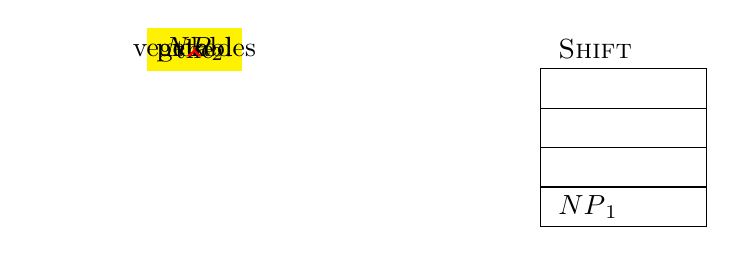
\begin{tikzpicture}
  \node at (-2, 0) {}; % force left edge here
  \Tree [.\node[fill=yellow,fill opacity=0,text opacity=1](S){\color{black} S};
          [.\node[fill=yellow,fill opacity=0,text opacity=1](NP1){\color{gray} $\text{NP}_1$};
            \node[fill=yellow,fill opacity=0,text opacity=1](The){\color{gray} The};
            \node[fill=yellow,fill opacity=0,text opacity=1](man){\color{gray} man}; ]
          [.\node[fill=yellow,fill opacity=0,text opacity=1]{\color{black} VP};
            [.\node[fill=yellow,fill opacity=1,text opacity=1](picked){\color{black} picked}; ]
            [.\node[fill=yellow,fill opacity=0,text opacity=1](NP2){\color{black} $\text{NP}_2$};
              \node[fill=yellow,fill opacity=0,text opacity=1]{\color{black} the};
              \node[fill=yellow,fill opacity=0,text opacity=1]{\color{black} vegetables}; ] ] ];
  \node [anchor=west] (cmd) at (4.5, 0) {\textsc{Shift}};
  \draw (4.4, -0.25) rectangle (6.5, -0.75);
  \draw (4.4, -0.75) rectangle (6.5, -1.25);
  \draw [fill=none] (4.4, -1.25) rectangle (6.5, -1.75);
  \draw [fill=none] (4.4, -1.75) rectangle (6.5, -2.25);
%  \node [anchor=west] (s4) at (4.5, -0.5) {vegetables};
%  \node [anchor=west] (s3) at (4.5, -1) {};
%  \node [anchor=west] (s2) at (4.5, -1.5) {The};
  \node [anchor=west] (s1) at (4.5, -2) {$\text{NP}_1$};
  \draw [->, thick, red] (The.center) -- (man.center);
  \draw [->, thick, red] (man.center) -- (NP1.center);
  \draw [->, thick, red] (NP1.center) -- (picked.center);
\end{tikzpicture}

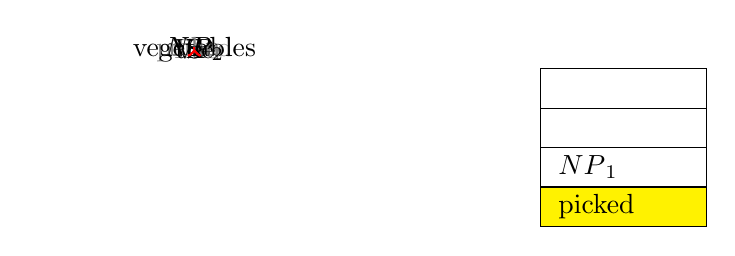
\begin{tikzpicture}
  \node at (-2, 0) {}; % force left edge here
  \Tree [.\node[fill=yellow,fill opacity=0,text opacity=1](S){\color{black} S};
          [.\node[fill=yellow,fill opacity=0,text opacity=1](NP1){\color{gray} $\text{NP}_1$};
            \node[fill=yellow,fill opacity=0,text opacity=1](The){\color{gray} The};
            \node[fill=yellow,fill opacity=0,text opacity=1](man){\color{gray} man}; ]
          [.\node[fill=yellow,fill opacity=0,text opacity=1]{\color{black} VP};
            [.\node[fill=yellow,fill opacity=0,text opacity=1](picked){\color{gray} picked}; ]
            [.\node[fill=yellow,fill opacity=0,text opacity=1](NP2){\color{black} $\text{NP}_2$};
              \node[fill=yellow,fill opacity=0,text opacity=1]{\color{black} the};
              \node[fill=yellow,fill opacity=0,text opacity=1]{\color{black} vegetables}; ] ] ];
%  \node [anchor=west] (cmd) at (4.5, 0) {\textsc{Shift}};
  \draw (4.4, -0.25) rectangle (6.5, -0.75);
  \draw (4.4, -0.75) rectangle (6.5, -1.25);
  \draw [fill=none] (4.4, -1.25) rectangle (6.5, -1.75);
  \draw [fill=yellow] (4.4, -1.75) rectangle (6.5, -2.25);
%  \node [anchor=west] (s4) at (4.5, -0.5) {vegetables};
%  \node [anchor=west] (s3) at (4.5, -1) {};
  \node [anchor=west] (s2) at (4.5, -1.5) {$\text{NP}_1$};
  \node [anchor=west] (s1) at (4.5, -2) {picked};
  \draw [->, thick, red] (The.center) -- (man.center);
  \draw [->, thick, red] (man.center) -- (NP1.center);
  \draw [->, thick, red] (NP1.center) -- (picked.center);
\end{tikzpicture}

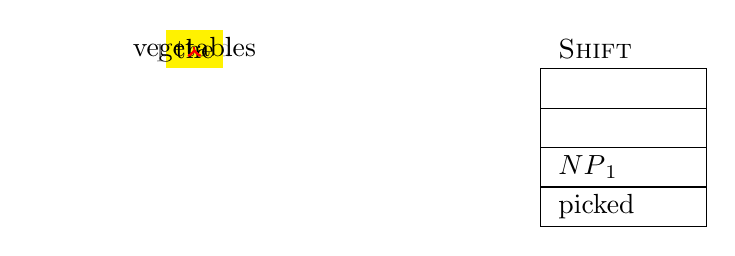
\begin{tikzpicture}
  \node at (-2, 0) {}; % force left edge here
  \Tree [.\node[fill=yellow,fill opacity=0,text opacity=1](S){\color{black} S};
          [.\node[fill=yellow,fill opacity=0,text opacity=1](NP1){\color{gray} $\text{NP}_1$};
            \node[fill=yellow,fill opacity=0,text opacity=1](The){\color{gray} The};
            \node[fill=yellow,fill opacity=0,text opacity=1](man){\color{gray} man}; ]
          [.\node[fill=yellow,fill opacity=0,text opacity=1]{\color{black} VP};
            [.\node[fill=yellow,fill opacity=0,text opacity=1](picked){\color{gray} picked}; ]
            [.\node[fill=yellow,fill opacity=0,text opacity=1](NP2){\color{black} $\text{NP}_2$};
              \node[fill=yellow,fill opacity=1,text opacity=1](the2){\color{black} the};
              \node[fill=yellow,fill opacity=0,text opacity=1]{\color{black} vegetables}; ] ] ];
  \node [anchor=west] (cmd) at (4.5, 0) {\textsc{Shift}};
  \draw (4.4, -0.25) rectangle (6.5, -0.75);
  \draw (4.4, -0.75) rectangle (6.5, -1.25);
  \draw [fill=none] (4.4, -1.25) rectangle (6.5, -1.75);
  \draw [fill=none] (4.4, -1.75) rectangle (6.5, -2.25);
%  \node [anchor=west] (s4) at (4.5, -0.5) {vegetables};
%  \node [anchor=west] (s3) at (4.5, -1) {};
  \node [anchor=west] (s2) at (4.5, -1.5) {$\text{NP}_1$};
  \node [anchor=west] (s1) at (4.5, -2) {picked};
  \draw [->, thick, red] (The.center) -- (man.center);
  \draw [->, thick, red] (man.center) -- (NP1.center);
  \draw [->, thick, red] (NP1.center) -- (picked.center);
  \draw [->, thick, red] (picked.center) -- (the2.center);
\end{tikzpicture}

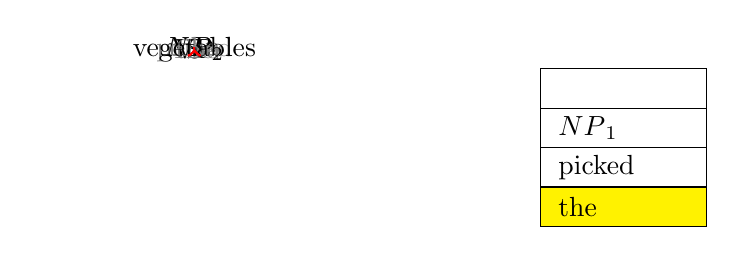
\begin{tikzpicture}
  \node at (-2, 0) {}; % force left edge here
  \Tree [.\node[fill=yellow,fill opacity=0,text opacity=1](S){\color{black} S};
          [.\node[fill=yellow,fill opacity=0,text opacity=1](NP1){\color{gray} $\text{NP}_1$};
            \node[fill=yellow,fill opacity=0,text opacity=1](The){\color{gray} The};
            \node[fill=yellow,fill opacity=0,text opacity=1](man){\color{gray} man}; ]
          [.\node[fill=yellow,fill opacity=0,text opacity=1]{\color{black} VP};
            [.\node[fill=yellow,fill opacity=0,text opacity=1](picked){\color{gray} picked}; ]
            [.\node[fill=yellow,fill opacity=0,text opacity=1](NP2){\color{black} $\text{NP}_2$};
              \node[fill=yellow,fill opacity=0,text opacity=1](the2){\color{gray} the};
              \node[fill=yellow,fill opacity=0,text opacity=1]{\color{black} vegetables}; ] ] ];
%  \node [anchor=west] (cmd) at (4.5, 0) {\textsc{Shift}};
  \draw (4.4, -0.25) rectangle (6.5, -0.75);
  \draw (4.4, -0.75) rectangle (6.5, -1.25);
  \draw [fill=none] (4.4, -1.25) rectangle (6.5, -1.75);
  \draw [fill=yellow] (4.4, -1.75) rectangle (6.5, -2.25);
%  \node [anchor=west] (s4) at (4.5, -0.5) {vegetables};
  \node [anchor=west] (s3) at (4.5, -1) {$\text{NP}_1$};
  \node [anchor=west] (s2) at (4.5, -1.5) {picked};
  \node [anchor=west] (s1) at (4.5, -2) {the};
  \draw [->, thick, red] (The.center) -- (man.center);
  \draw [->, thick, red] (man.center) -- (NP1.center);
  \draw [->, thick, red] (NP1.center) -- (picked.center);
  \draw [->, thick, red] (picked.center) -- (the2.center);
\end{tikzpicture}

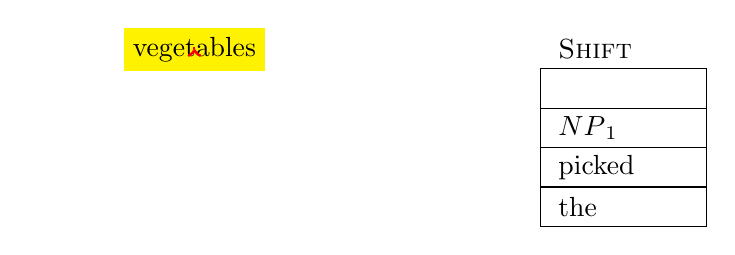
\begin{tikzpicture}
  \node at (-2, 0) {}; % force left edge here
  \Tree [.\node[fill=yellow,fill opacity=0,text opacity=1](S){\color{black} S};
          [.\node[fill=yellow,fill opacity=0,text opacity=1](NP1){\color{gray} $\text{NP}_1$};
            \node[fill=yellow,fill opacity=0,text opacity=1](The){\color{gray} The};
            \node[fill=yellow,fill opacity=0,text opacity=1](man){\color{gray} man}; ]
          [.\node[fill=yellow,fill opacity=0,text opacity=1]{\color{black} VP};
            [.\node[fill=yellow,fill opacity=0,text opacity=1](picked){\color{gray} picked}; ]
            [.\node[fill=yellow,fill opacity=0,text opacity=1](NP2){\color{black} $\text{NP}_2$};
              \node[fill=yellow,fill opacity=0,text opacity=1](the2){\color{gray} the};
              \node[fill=yellow,fill opacity=1,text opacity=1](vegetables){\color{black} vegetables}; ] ] ];
  \node [anchor=west] (cmd) at (4.5, 0) {\textsc{Shift}};
  \draw (4.4, -0.25) rectangle (6.5, -0.75);
  \draw (4.4, -0.75) rectangle (6.5, -1.25);
  \draw [fill=none] (4.4, -1.25) rectangle (6.5, -1.75);
  \draw [fill=none] (4.4, -1.75) rectangle (6.5, -2.25);
%  \node [anchor=west] (s4) at (4.5, -0.5) {vegetables};
  \node [anchor=west] (s3) at (4.5, -1) {$\text{NP}_1$};
  \node [anchor=west] (s2) at (4.5, -1.5) {picked};
  \node [anchor=west] (s1) at (4.5, -2) {the};
  \draw [->, thick, red] (The.center) -- (man.center);
  \draw [->, thick, red] (man.center) -- (NP1.center);
  \draw [->, thick, red] (NP1.center) -- (picked.center);
  \draw [->, thick, red] (picked.center) -- (the2.center);
  \draw [->, thick, red] (the2.center) -- (vegetables.center);
\end{tikzpicture}

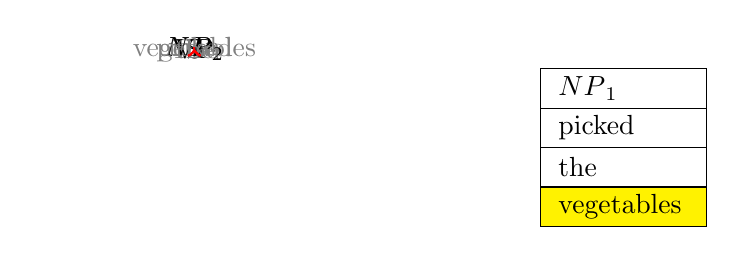
\begin{tikzpicture}
  \node at (-2, 0) {}; % force left edge here
  \Tree [.\node[fill=yellow,fill opacity=0,text opacity=1](S){\color{black} S};
          [.\node[fill=yellow,fill opacity=0,text opacity=1](NP1){\color{gray} $\text{NP}_1$};
            \node[fill=yellow,fill opacity=0,text opacity=1](The){\color{gray} The};
            \node[fill=yellow,fill opacity=0,text opacity=1](man){\color{gray} man}; ]
          [.\node[fill=yellow,fill opacity=0,text opacity=1]{\color{black} VP};
            [.\node[fill=yellow,fill opacity=0,text opacity=1](picked){\color{gray} picked}; ]
            [.\node[fill=yellow,fill opacity=0,text opacity=1](NP2){\color{black} $\text{NP}_2$};
              \node[fill=yellow,fill opacity=0,text opacity=1](the2){\color{gray} the};
              \node[fill=yellow,fill opacity=0,text opacity=1](vegetables){\color{gray} vegetables}; ] ] ];
%  \node [anchor=west] (cmd) at (4.5, 0) {\textsc{Shift}};
  \draw (4.4, -0.25) rectangle (6.5, -0.75);
  \draw (4.4, -0.75) rectangle (6.5, -1.25);
  \draw [fill=none] (4.4, -1.25) rectangle (6.5, -1.75);
  \draw [fill=yellow] (4.4, -1.75) rectangle (6.5, -2.25);
  \node [anchor=west] (s4) at (4.5, -0.5) {$\text{NP}_1$};
  \node [anchor=west] (s3) at (4.5, -1) {picked};
  \node [anchor=west] (s2) at (4.5, -1.5) {the};
  \node [anchor=west] (s1) at (4.5, -2) {vegetables};
  \draw [->, thick, red] (The.center) -- (man.center);
  \draw [->, thick, red] (man.center) -- (NP1.center);
  \draw [->, thick, red] (NP1.center) -- (picked.center);
  \draw [->, thick, red] (picked.center) -- (the2.center);
  \draw [->, thick, red] (the2.center) -- (vegetables.center);
\end{tikzpicture}

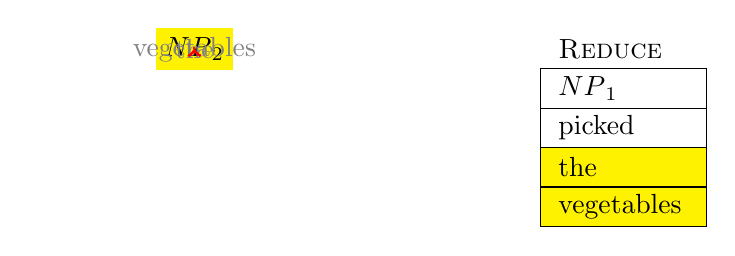
\begin{tikzpicture}
  \node at (-2, 0) {}; % force left edge here
  \Tree [.\node[fill=yellow,fill opacity=0,text opacity=1](S){\color{black} S};
          [.\node[fill=yellow,fill opacity=0,text opacity=1](NP1){\color{gray} $\text{NP}_1$};
            \node[fill=yellow,fill opacity=0,text opacity=1](The){\color{gray} The};
            \node[fill=yellow,fill opacity=0,text opacity=1](man){\color{gray} man}; ]
          [.\node[fill=yellow,fill opacity=0,text opacity=1]{\color{black} VP};
            [.\node[fill=yellow,fill opacity=0,text opacity=1](picked){\color{gray} picked}; ]
            [.\node[fill=yellow,fill opacity=1,text opacity=1](NP2){\color{black} $\text{NP}_2$};
              \node[fill=yellow,fill opacity=0,text opacity=1](the2){\color{gray} the};
              \node[fill=yellow,fill opacity=0,text opacity=1](vegetables){\color{gray} vegetables}; ] ] ];
  \node [anchor=west] (cmd) at (4.5, 0) {\textsc{Reduce}};
  \draw (4.4, -0.25) rectangle (6.5, -0.75);
  \draw (4.4, -0.75) rectangle (6.5, -1.25);
  \draw [fill=yellow] (4.4, -1.25) rectangle (6.5, -1.75);
  \draw [fill=yellow] (4.4, -1.75) rectangle (6.5, -2.25);
  \node [anchor=west] (s4) at (4.5, -0.5) {$\text{NP}_1$};
  \node [anchor=west] (s3) at (4.5, -1) {picked};
  \node [anchor=west] (s2) at (4.5, -1.5) {the};
  \node [anchor=west] (s1) at (4.5, -2) {vegetables};
  \draw [->, thick, red] (The.center) -- (man.center);
  \draw [->, thick, red] (man.center) -- (NP1.center);
  \draw [->, thick, red] (NP1.center) -- (picked.center);
  \draw [->, thick, red] (picked.center) -- (the2.center);
  \draw [->, thick, red] (the2.center) -- (vegetables.center);
  \draw [->, thick, red] (vegetables.center) -- (NP2.center);
\end{tikzpicture}

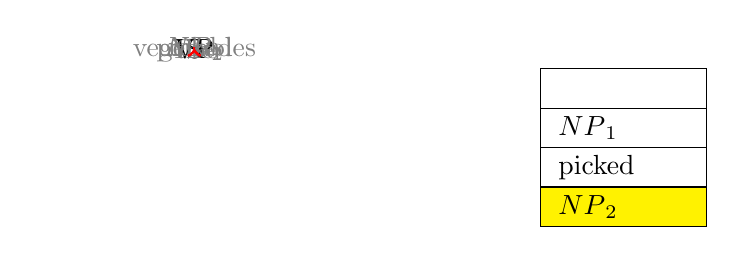
\begin{tikzpicture}
  \node at (-2, 0) {}; % force left edge here
  \Tree [.\node[fill=yellow,fill opacity=0,text opacity=1](S){\color{black} S};
          [.\node[fill=yellow,fill opacity=0,text opacity=1](NP1){\color{gray} $\text{NP}_1$};
            \node[fill=yellow,fill opacity=0,text opacity=1](The){\color{gray} The};
            \node[fill=yellow,fill opacity=0,text opacity=1](man){\color{gray} man}; ]
          [.\node[fill=yellow,fill opacity=0,text opacity=1]{\color{black} VP};
            [.\node[fill=yellow,fill opacity=0,text opacity=1](picked){\color{gray} picked}; ]
            [.\node[fill=yellow,fill opacity=0,text opacity=1](NP2){\color{gray} $\text{NP}_2$};
              \node[fill=yellow,fill opacity=0,text opacity=1](the2){\color{gray} the};
              \node[fill=yellow,fill opacity=0,text opacity=1](vegetables){\color{gray} vegetables}; ] ] ];
%  \node [anchor=west] (cmd) at (4.5, 0) {\textsc{Reduce}};
  \draw (4.4, -0.25) rectangle (6.5, -0.75);
  \draw (4.4, -0.75) rectangle (6.5, -1.25);
  \draw [fill=none] (4.4, -1.25) rectangle (6.5, -1.75);
  \draw [fill=yellow] (4.4, -1.75) rectangle (6.5, -2.25);
%  \node [anchor=west] (s4) at (4.5, -0.5) {};
  \node [anchor=west] (s3) at (4.5, -1) {$\text{NP}_1$};
  \node [anchor=west] (s2) at (4.5, -1.5) {picked};
  \node [anchor=west] (s1) at (4.5, -2) {$\text{NP}_2$};
  \draw [->, thick, red] (The.center) -- (man.center);
  \draw [->, thick, red] (man.center) -- (NP1.center);
  \draw [->, thick, red] (NP1.center) -- (picked.center);
  \draw [->, thick, red] (picked.center) -- (the2.center);
  \draw [->, thick, red] (the2.center) -- (vegetables.center);
  \draw [->, thick, red] (vegetables.center) -- (NP2.center);
\end{tikzpicture}

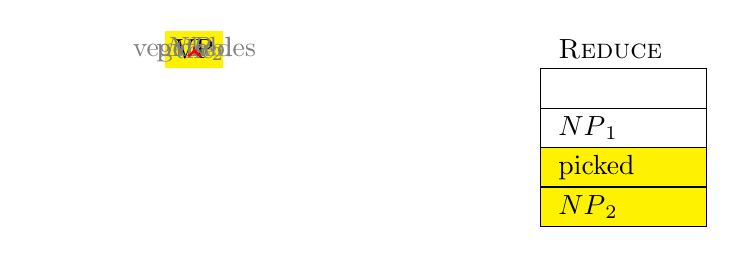
\begin{tikzpicture}
  \node at (-2, 0) {}; % force left edge here
  \Tree [.\node[fill=yellow,fill opacity=0,text opacity=1](S){\color{black} S};
          [.\node[fill=yellow,fill opacity=0,text opacity=1](NP1){\color{gray} $\text{NP}_1$};
            \node[fill=yellow,fill opacity=0,text opacity=1](The){\color{gray} The};
            \node[fill=yellow,fill opacity=0,text opacity=1](man){\color{gray} man}; ]
          [.\node[fill=yellow,fill opacity=1,text opacity=1](VP){\color{black} VP};
            [.\node[fill=yellow,fill opacity=0,text opacity=1](picked){\color{gray} picked}; ]
            [.\node[fill=yellow,fill opacity=0,text opacity=1](NP2){\color{gray} $\text{NP}_2$};
              \node[fill=yellow,fill opacity=0,text opacity=1](the2){\color{gray} the};
              \node[fill=yellow,fill opacity=0,text opacity=1](vegetables){\color{gray} vegetables}; ] ] ];
  \node [anchor=west] (cmd) at (4.5, 0) {\textsc{Reduce}};
  \draw (4.4, -0.25) rectangle (6.5, -0.75);
  \draw (4.4, -0.75) rectangle (6.5, -1.25);
  \draw [fill=yellow] (4.4, -1.25) rectangle (6.5, -1.75);
  \draw [fill=yellow] (4.4, -1.75) rectangle (6.5, -2.25);
%  \node [anchor=west] (s4) at (4.5, -0.5) {};
  \node [anchor=west] (s3) at (4.5, -1) {$\text{NP}_1$};
  \node [anchor=west] (s2) at (4.5, -1.5) {picked};
  \node [anchor=west] (s1) at (4.5, -2) {$\text{NP}_2$};
  \draw [->, thick, red] (The.center) -- (man.center);
  \draw [->, thick, red] (man.center) -- (NP1.center);
  \draw [->, thick, red] (NP1.center) -- (picked.center);
  \draw [->, thick, red] (picked.center) -- (the2.center);
  \draw [->, thick, red] (the2.center) -- (vegetables.center);
  \draw [->, thick, red] (vegetables.center) -- (NP2.center);
  \draw [->, thick, red] (NP2.center) -- (VP.center);
\end{tikzpicture}

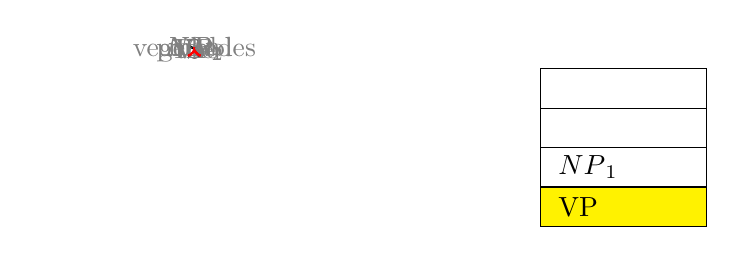
\begin{tikzpicture}
  \node at (-2, 0) {}; % force left edge here
  \Tree [.\node[fill=yellow,fill opacity=0,text opacity=1](S){\color{black} S};
          [.\node[fill=yellow,fill opacity=0,text opacity=1](NP1){\color{gray} $\text{NP}_1$};
            \node[fill=yellow,fill opacity=0,text opacity=1](The){\color{gray} The};
            \node[fill=yellow,fill opacity=0,text opacity=1](man){\color{gray} man}; ]
          [.\node[fill=yellow,fill opacity=0,text opacity=1](VP){\color{gray} VP};
            [.\node[fill=yellow,fill opacity=0,text opacity=1](picked){\color{gray} picked}; ]
            [.\node[fill=yellow,fill opacity=0,text opacity=1](NP2){\color{gray} $\text{NP}_2$};
              \node[fill=yellow,fill opacity=0,text opacity=1](the2){\color{gray} the};
              \node[fill=yellow,fill opacity=0,text opacity=1](vegetables){\color{gray} vegetables}; ] ] ];
%  \node [anchor=west] (cmd) at (4.5, 0) {\textsc{Reduce}};
  \draw (4.4, -0.25) rectangle (6.5, -0.75);
  \draw (4.4, -0.75) rectangle (6.5, -1.25);
  \draw [fill=none] (4.4, -1.25) rectangle (6.5, -1.75);
  \draw [fill=yellow] (4.4, -1.75) rectangle (6.5, -2.25);
%  \node [anchor=west] (s4) at (4.5, -0.5) {};
%  \node [anchor=west] (s3) at (4.5, -1) {};
  \node [anchor=west] (s2) at (4.5, -1.5) {$\text{NP}_1$};
  \node [anchor=west] (s1) at (4.5, -2) {VP};
  \draw [->, thick, red] (The.center) -- (man.center);
  \draw [->, thick, red] (man.center) -- (NP1.center);
  \draw [->, thick, red] (NP1.center) -- (picked.center);
  \draw [->, thick, red] (picked.center) -- (the2.center);
  \draw [->, thick, red] (the2.center) -- (vegetables.center);
  \draw [->, thick, red] (vegetables.center) -- (NP2.center);
  \draw [->, thick, red] (NP2.center) -- (VP.center);
\end{tikzpicture}

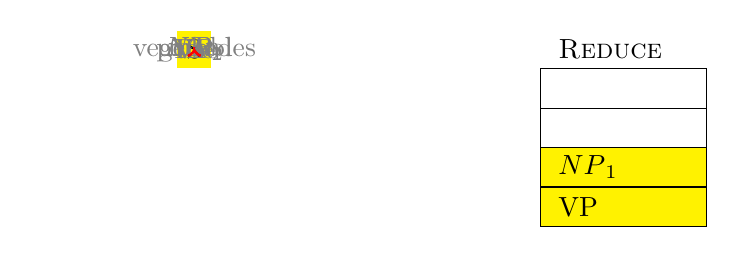
\begin{tikzpicture}
  \node at (-2, 0) {}; % force left edge here
  \Tree [.\node[fill=yellow,fill opacity=1,text opacity=1](S){\color{black} S};
          [.\node[fill=yellow,fill opacity=0,text opacity=1](NP1){\color{gray} $\text{NP}_1$};
            \node[fill=yellow,fill opacity=0,text opacity=1](The){\color{gray} The};
            \node[fill=yellow,fill opacity=0,text opacity=1](man){\color{gray} man}; ]
          [.\node[fill=yellow,fill opacity=0,text opacity=1](VP){\color{gray} VP};
            [.\node[fill=yellow,fill opacity=0,text opacity=1](picked){\color{gray} picked}; ]
            [.\node[fill=yellow,fill opacity=0,text opacity=1](NP2){\color{gray} $\text{NP}_2$};
              \node[fill=yellow,fill opacity=0,text opacity=1](the2){\color{gray} the};
              \node[fill=yellow,fill opacity=0,text opacity=1](vegetables){\color{gray} vegetables}; ] ] ];
  \node [anchor=west] (cmd) at (4.5, 0) {\textsc{Reduce}};
  \draw (4.4, -0.25) rectangle (6.5, -0.75);
  \draw (4.4, -0.75) rectangle (6.5, -1.25);
  \draw [fill=yellow] (4.4, -1.25) rectangle (6.5, -1.75);
  \draw [fill=yellow] (4.4, -1.75) rectangle (6.5, -2.25);
%  \node [anchor=west] (s4) at (4.5, -0.5) {};
%  \node [anchor=west] (s3) at (4.5, -1) {};
  \node [anchor=west] (s2) at (4.5, -1.5) {$\text{NP}_1$};
  \node [anchor=west] (s1) at (4.5, -2) {VP};
  \draw [->, thick, red] (The.center) -- (man.center);
  \draw [->, thick, red] (man.center) -- (NP1.center);
  \draw [->, thick, red] (NP1.center) -- (picked.center);
  \draw [->, thick, red] (picked.center) -- (the2.center);
  \draw [->, thick, red] (the2.center) -- (vegetables.center);
  \draw [->, thick, red] (vegetables.center) -- (NP2.center);
  \draw [->, thick, red] (NP2.center) -- (VP.center);
  \draw [->, thick, red] (VP.center) -- (S.center);
\end{tikzpicture}